% !TEX root = ../main.tex
%--- Slide 6: la degenerazione DM-scattering (circa 1 min 15 s) --------------------------
% Figura: Figure/P06_reali_DM_SV.pdf (notebook 26), solo dati reali DR2low.
\begin{frame}{La degenerazione DM--scattering}
  \begin{columns}[c]
    \column{0.45\textwidth}
    \centering
    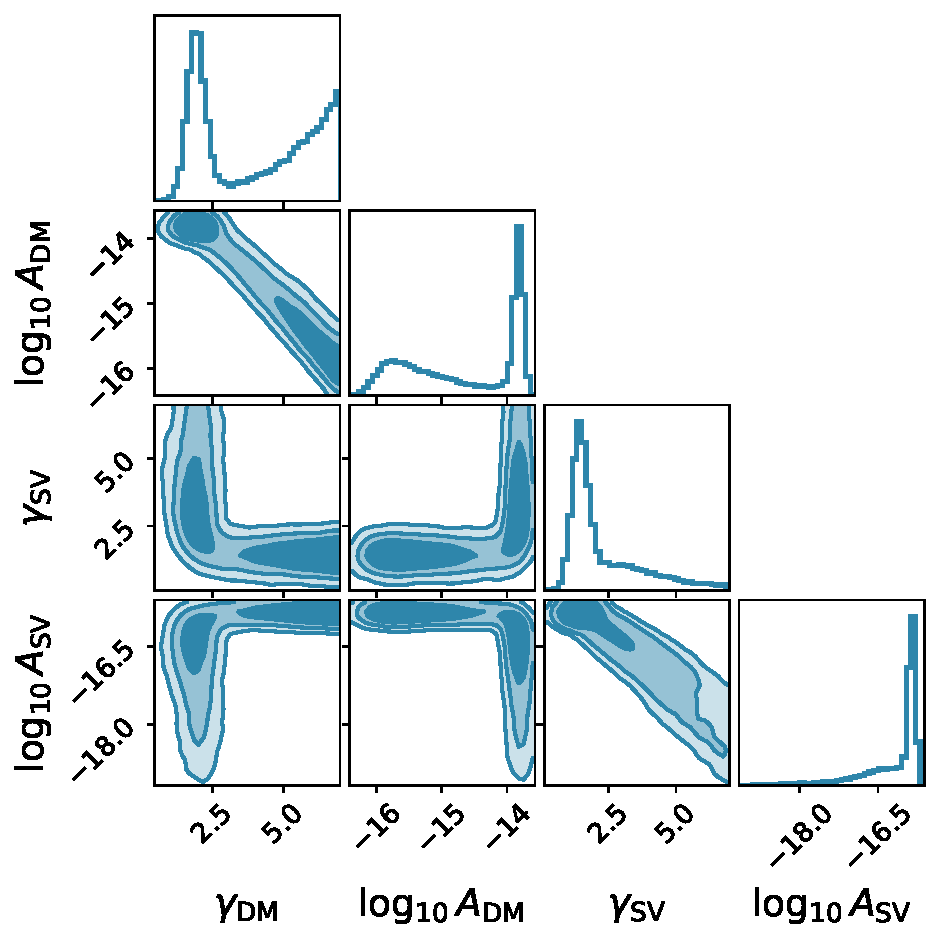
\includegraphics[height=0.82\textheight]{Figure/P06_reali_DM_SV.pdf}
    \column{0.52\textwidth}
    \begin{itemize}
      \item Il DM ha \textbf{due picchi}:
        \begin{itemize}
          \item ampiezza alta: $\log_{10}A_{\rm DM} \simeq -13.8$, $\gamma_{\rm DM} \simeq 2$
          \item ampiezza bassa: $\log_{10}A_{\rm DM} \simeq -15.5$, $\gamma_{\rm DM}$ al bordo del prior
        \end{itemize}
      \item Tra DM e scattering i contorni hanno \textbf{forma a L}
      \item Il rumore cromatico si descrive con il DM \emph{o} con lo scattering:
            i dati non scelgono
    \end{itemize}
  \end{columns}
\end{frame}
